\documentclass[11pt,a4paper]{article}
\usepackage{algorithm, algorithmic, listings} % Code
\usepackage{amsmath, amstext, amssymb, amsfonts, dsfont, cancel, mathtools} % Math
\usepackage{color, xcolor} % Color
\usepackage{diagbox, tabularx} % Table
\usepackage{enumerate} % List
\usepackage{epsfig, epstopdf, graphicx, multicol, multirow, palatino, pgfplots, subcaption, tikz} % Image.
\usepackage{fancybox}
\usepackage{verbatim}

\usepackage[font=footnotesize]{caption} % labelfont=bf
\usepackage[font=scriptsize]{subcaption} % labelfont=bf
\usepackage[margin=1in]{geometry}
\usepackage[hidelinks]{hyperref}
\epstopdfsetup{outdir=./Figure/Converted/}
\graphicspath{{./Figure/}}

\makeatletter
\def\input@path{{./Figure/}}
\makeatother

\pgfplotsset{compat=1.13} 

% MATLAB code settings
\lstset{extendedchars=false, % Shutdown no-ASCII compatible
basicstyle=\normalsize\tt, % the size of the fonts that are used for the code
language=Matlab, tabsize=4, numbers=left, numberstyle=\small, stepnumber=1, numbersep=8pt, keywordstyle=\color[rgb]{0,0,1}, commentstyle=\color[rgb]{0.133,0.545,0.133}, stringstyle=\color[rgb]{0.627,0.126,0.941}, backgroundcolor=\color{white}, showspaces=false, showstringspaces=false, showtabs=false, frame=single, captionpos=t, breaklines=true, breakatwhitespace=false, morekeywords={break, case, catch, continue, elseif, else, end, for, function, global, if, otherwise, persistent, return, switch, try, while}, title=\lstname,
mathescape=true,escapechar=? % escape to latex with ?..?  
escapeinside={\%*}{*)}, % if you want to add a comment within your code  
%morestring=[m]', % strings
%columns=fixed, % nice spacing
}

\begin{document}
\title{\sc\vspace{3cm}\hrule\vspace{0.3cm}{\LARGE DD2423}\\\vspace{0.1cm}{\Large Image Analysis and Computer Vision}\vspace{0.3cm}\hrule\vspace{1.5cm}{\Large Laboratory Report}\\{\large Lab 3: Image Segmentation}}
\author{Jiang, Sifan\\sifanj@kth.se}
\maketitle
\newpage

\newcounter{Counter}
\setcounter{Counter}{0}
%\item\addtocounter{Counter}{1}\textbf{Question \arabic{Counter}:}

\section{K-meas clustering}
\begin{itemize}
	\item\addtocounter{Counter}{1}\underline{\textbf{Question \arabic{Counter}:}} How did you initialize the clustering process and why do you believe this was a good method of doing it?
		\par Since we have priori information with the image \texttt{orange} and based on the image, the main colors in the image are white, which is the background and the textures of the oranges, orange, which is the oranges themselves, and gray, which is the shadow of the oranges. So, we can set the centers based on these three colors.
		\par However, if we don't know the priori information and that's how we implement the code, the best way to initialize the clustering process is to chose the centers randomly.

	\item\addtocounter{Counter}{1}\underline{\textbf{Question \arabic{Counter}:}} How many iterations \texttt{L} do you typically need to reach convergence, that is the point where no additional iterations will affect the end results?
		\par The number of iterations depends on the number of clusters \texttt{K}, the number of the pixels, the initial cluster centers and the complexity of the image. In our case, the blurring degree could also affect the iteration amount.
		\par For \texttt{orange}, we typically need iteration time varies from $10$ to $30$ times to obtain a nice result of segmentation(clear boundary between two halves of the orange). The specific number of iteration would change according to the parameter setting.

	\item\addtocounter{Counter}{1}\underline{\textbf{Question \arabic{Counter}:}} What is the minimum value for \texttt{K} that you can use and still get no superpixel that covers parts from both halves of the orange? Illustrate with a figure.
		\par From figure \ref{fig:Kmeans_Orange_K_16_L_X} and \ref{fig:Kmeans_Orange_K_17_L_X}, the minimum value for \texttt{K} to get no superpixels that covers parts form both halves of the orange in my implementation is $17$. When \texttt{K} is $16$, there is no boundary between two halves of the orange, while if \texttt{K} is $17$, there exists a clear boundary.\
		\par In this case, I still use the default value for $\sigma=1.0$ which is the image preblurring scale. If this value is smaller, then the minimum \texttt{K} to have obvious boundary between two halves of the orange could decrease.
		\begin{figure}[!ht]
			\centering
			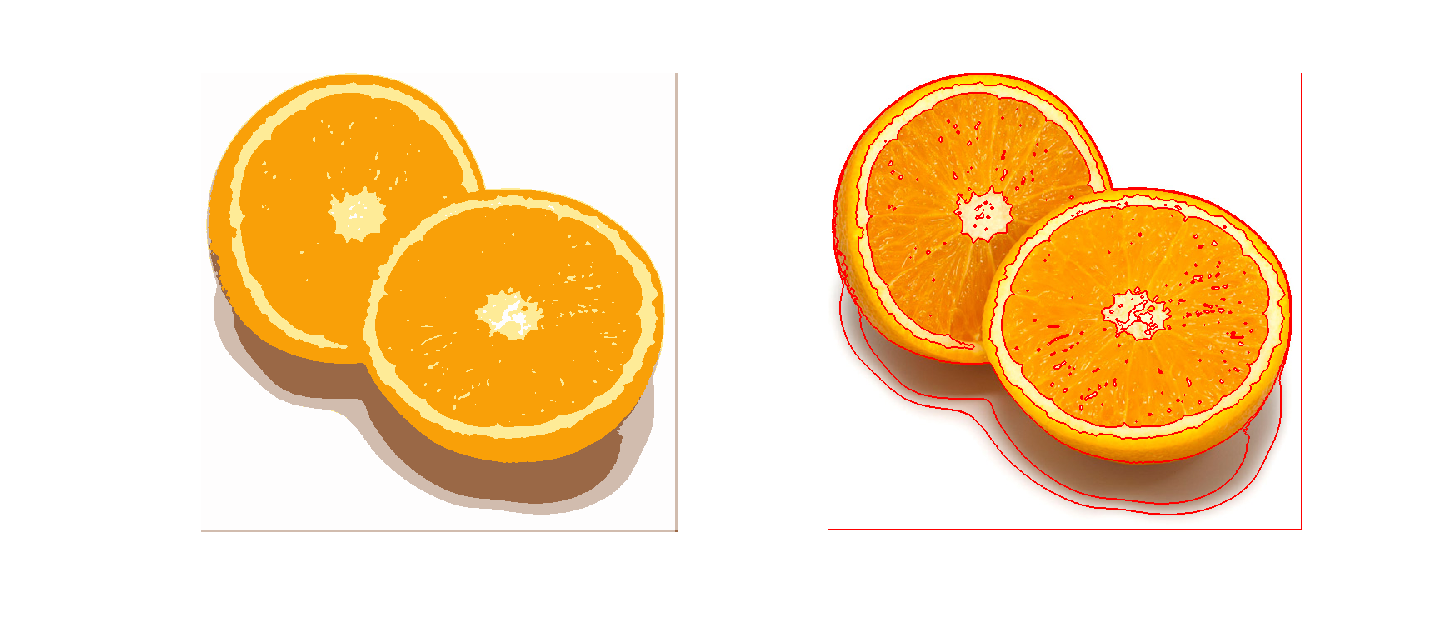
\includegraphics[width=\columnwidth]{Kmeans_Orange_K_16_L_X.eps}
			\caption{Segmented \texttt{orange} with 16 clusters.}
			\label{fig:Kmeans_Orange_K_16_L_X}
		\end{figure}
		
		\begin{figure}[!ht]
			\centering
			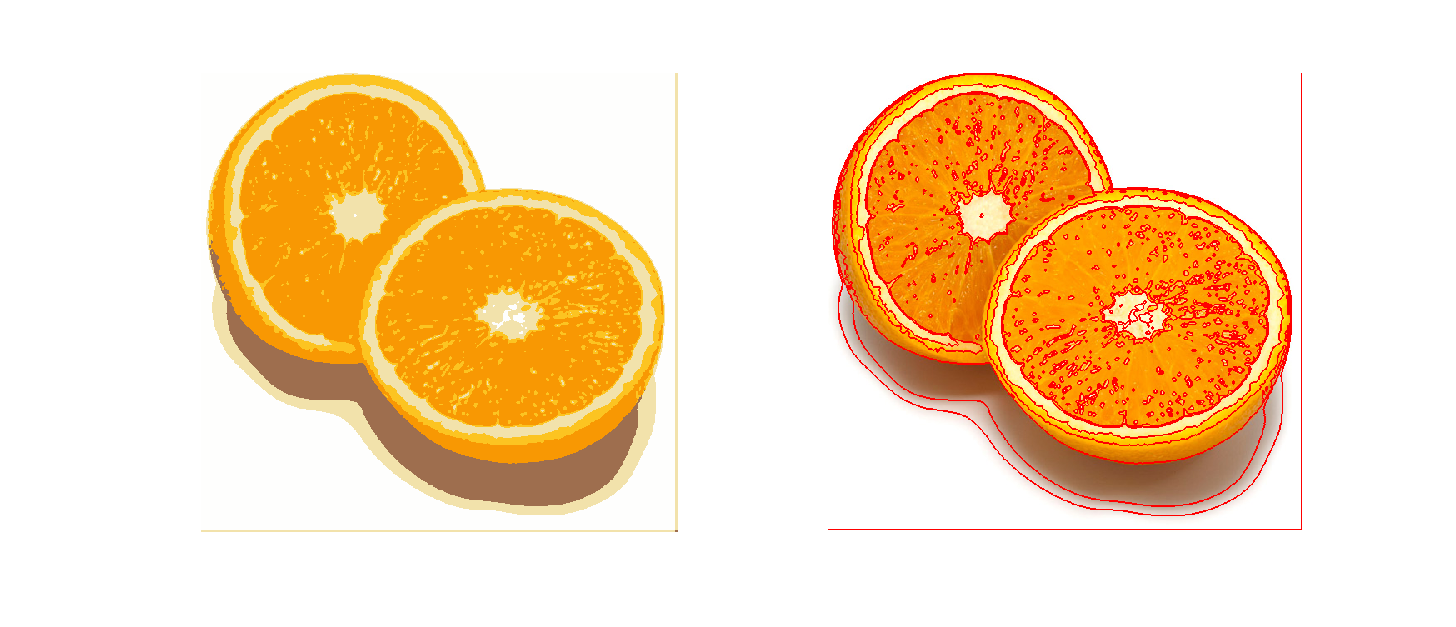
\includegraphics[width=\columnwidth]{Kmeans_Orange_K_17_L_X.eps}
			\caption{Segmented \texttt{orange} with 17 clusters.}
			\label{fig:Kmeans_Orange_K_17_L_X}
		\end{figure}

	\item\addtocounter{Counter}{1}\underline{\textbf{Question \arabic{Counter}:}} What needs to be changed in the parameters to get suitable superpixels for the tiger images as well?
		\par We need to increase the cluster number \texttt{K} since the images \texttt{tiger} are more complex than \texttt{orange} which have more color and details. Also, it would need more number of iterations, so the iteration time \texttt{L} should be increased at the same time.

\end{itemize}

\section{Mean-shift segmentation}
\begin{itemize}
	\item\addtocounter{Counter}{1}\underline{\textbf{Question \arabic{Counter}:}} How do the results change depending on the bandwidths? What settings did you prefer for the different images? Illustrate with an example image with the parameter that you think are suitable for that image.
	\par The spatial bandwidth $\sigma_{s}^{2}$ is responsible for the range of the density function around pixels in $5$ dimension spatial and color space. As $\sigma_{s}^{2}$ increases, the range of the Gaussian increases, thus the density function spread over more space and more likely to mix with other pixels. So, more pixels would be assigned to same mode and the number of modes decreases. Also, the spatial bandwidth determines the area of the segmentations. The larger the spatial bandwidth is, the larger the area of the segmentations could be, thus the less the number of modes would obtained.
	\par When the color bandwidth $\sigma_{c}^{2}$ increase, the diversity of color information of modes would decreases. Also, the overall color information would be more similar to the original image.
	\par For image \texttt{tiger\_1}, the best parameters setting is spatial bandwidth equals to $4$ and color bandwidth equals to $2$, which is illustrated in Figure \ref{fig:Meanshift_Tiger1_Best_Result_S_4_C_2}.
	\begin{figure}[!ht]
		\centering
		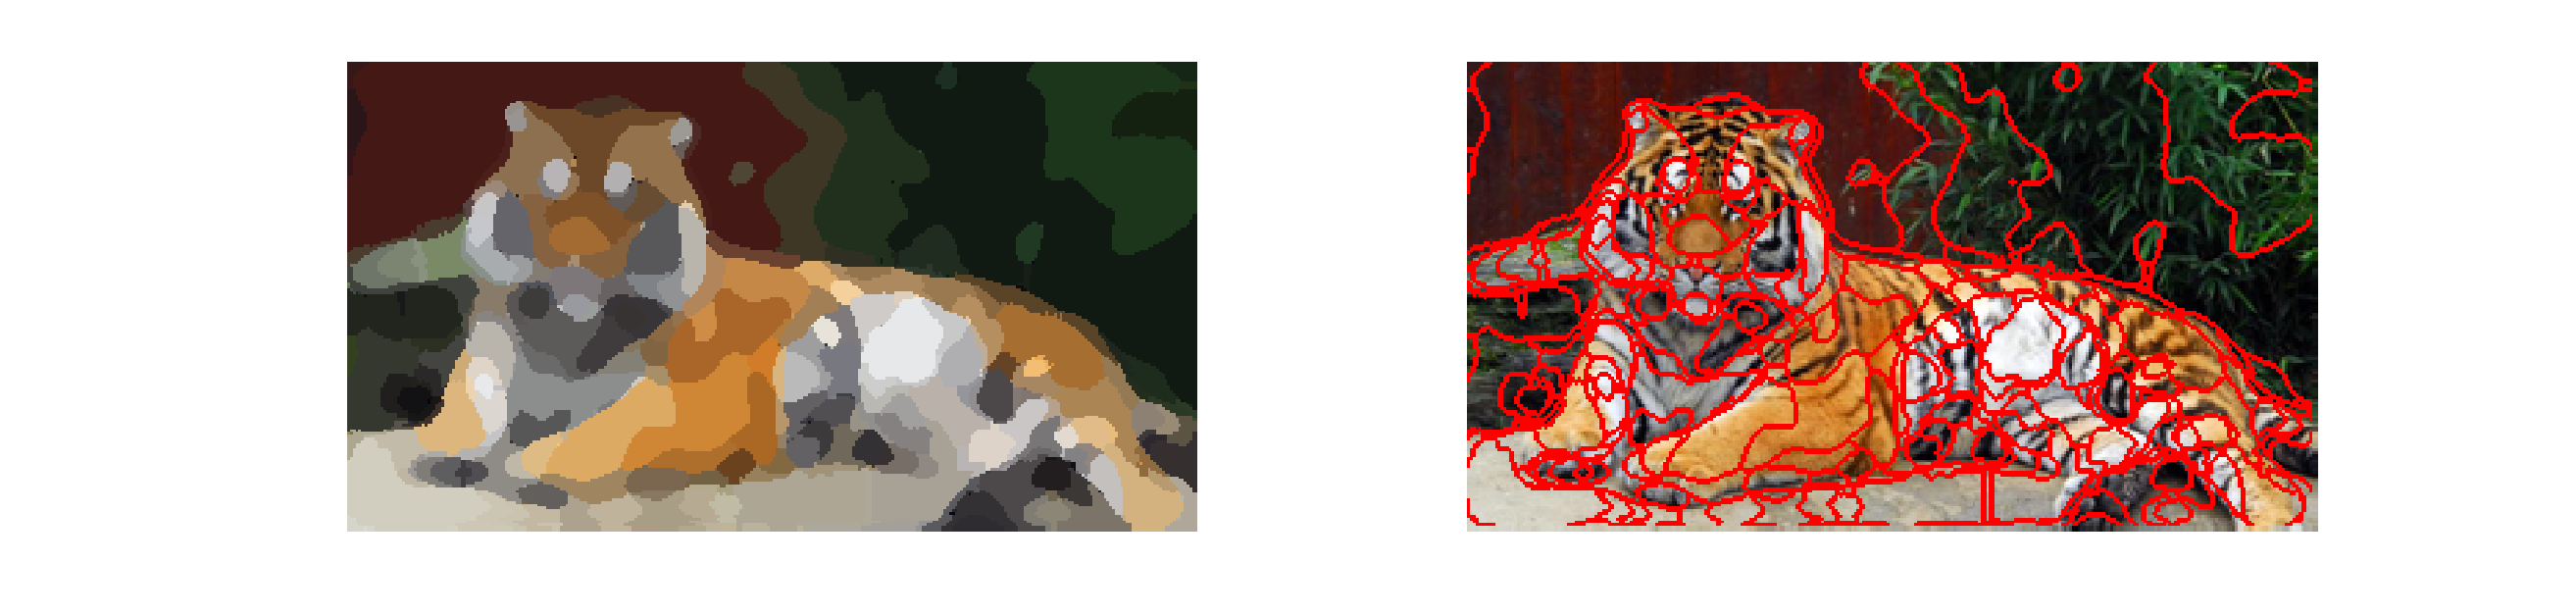
\includegraphics[width=\columnwidth]{Meanshift_Tiger1_Best_Result_S_4_C_2.eps}
		\caption{Best result for Mean-shift segmented \texttt{tiger\_1} with spatial bandwidth $4$ and color bandwidth $2$.}
		\label{fig:Meanshift_Tiger1_Best_Result_S_4_C_2}
	\end{figure}
	
	\item\addtocounter{Counter}{1}\underline{\textbf{Question \arabic{Counter}:}} What kind of similarities and differences do you see between K-means and mean-shift segmentation?
		\par K-means and mean-shift segmentation are both treat with the color and position of pixels and are to find the cluster centers and modes.
		\par However, mean-shift segmentation would not determine the number of modes before the segmentation start, which is different from K-means segmentation. Also, in our implementation, spatial information of the pixels is not taken into consideration in K-means segmentation. While mean-shift segmentation considers both spatial and color information.
	
\end{itemize}

\section{Normalized Cut}
\begin{itemize}
	\item\addtocounter{Counter}{1}\underline{\textbf{Question \arabic{Counter}:}} Does the ideal parameter setting vary depending on the images? If you look at the images, can you see a reason why the ideal settings might differ? Illustrate with an example image using the parameters you prefer for that image.
		\par The ideal parameter setting varies depending on the images. Figure \ref{fig:Normalizedcut_Tiger2_Default} shows the default parameters setting for Normalized Cut segmenting the image \texttt{tiger2}, with parameters noted in the title.

		\begin{figure}[!ht]
			\centering
			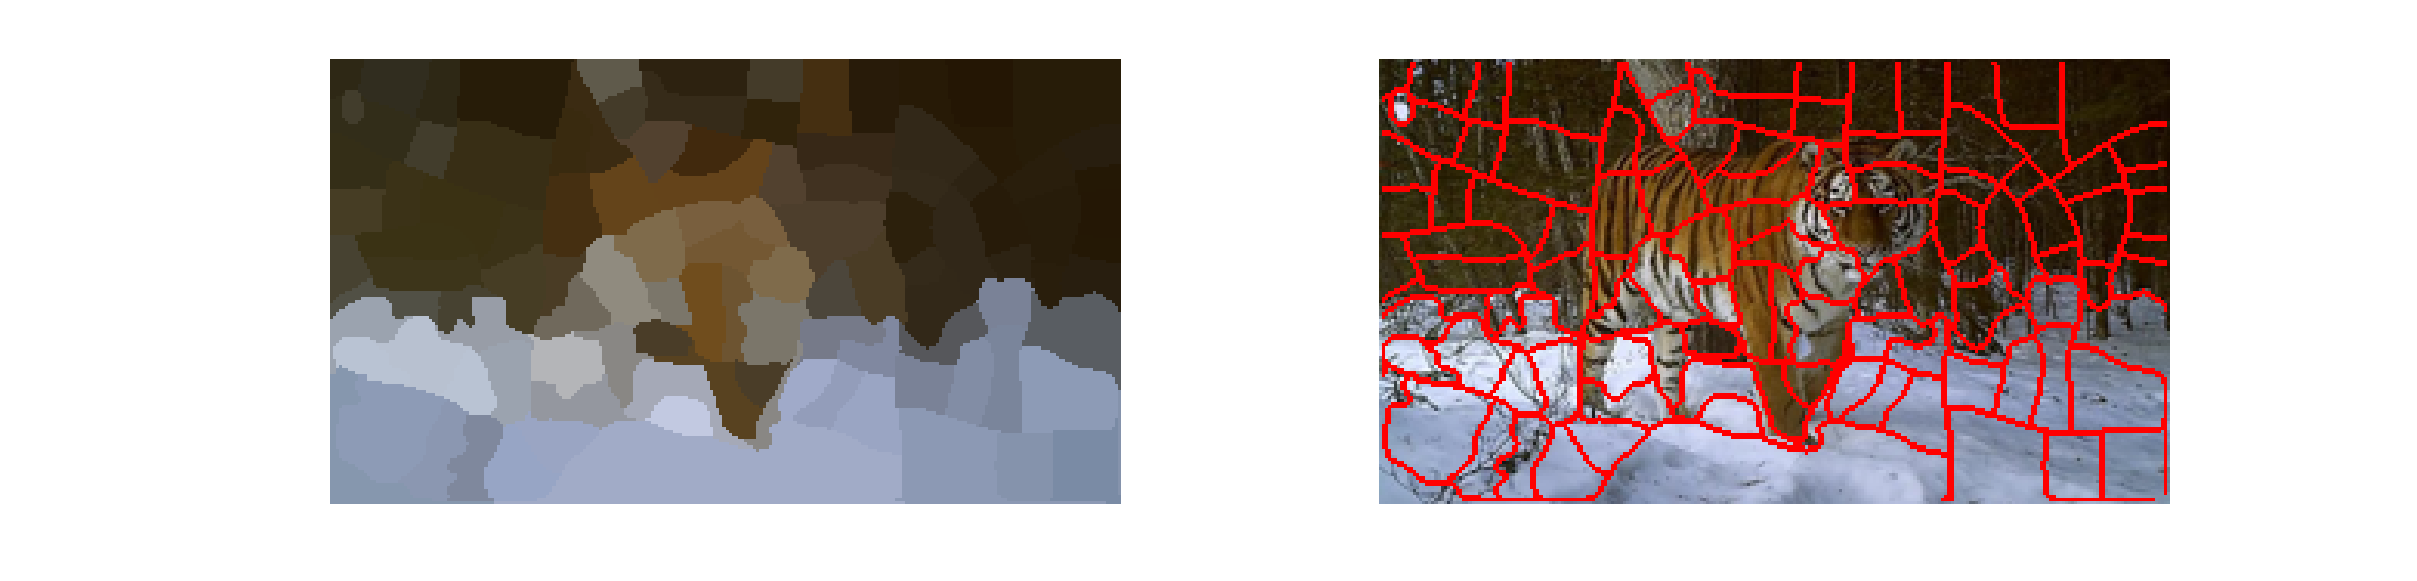
\includegraphics[width=\columnwidth]{Figure/Normalizedcut_Tiger2_Default.eps}
			\caption{Normalized Cut segmented \texttt{tiger2} with default parameters setting: \texttt{colour\_bandwidth} = $20.0$, \texttt{radius} = $3$, \texttt{ncuts\_thresh} = $0.2$, \texttt{min\_area} = $200$, and \texttt{max\_depth} = $8$.}
			\label{fig:Normalizedcut_Tiger2_Default}
		\end{figure}

		\par \texttt{ncut\_thresh} determines the color diversity of the result. The choice of \texttt{ncut\_thresh} depends on the overall complexity of the image. As illustrated in Figure \ref{fig:Normalizedcut_Tiger2_nCutsthresh_0_02}, the decrease of the maximum allowed value for a cut would result in the decrease the color diversity of the segmented image.

		\begin{figure}[!ht]
			\centering
			
\includegraphics[width=\columnwidth]{Figure/Normalizedcut_Tiger2_nCutsthresh_0_02.eps}
			\caption{Normalized Cut segmented \texttt{tiger2} with changing \texttt{ncuts\_thresh} to $0.02$.}
			\label{fig:Normalizedcut_Tiger2_nCutsthresh_0_02}
		\end{figure}

		\par \texttt{min\_area} determines the minimum size of each segmentation, so the choice of \texttt{min\_area} depends on the size of the image, the size of the complexity of the objects in the image. As shown in Figure \ref{fig:Normalizedcut_Tiger2_Minarea_20}, the decrease of \texttt{min\_area} would result in the decrease of segmented areas and more modes.

		\begin{figure}[!ht]
			\centering
			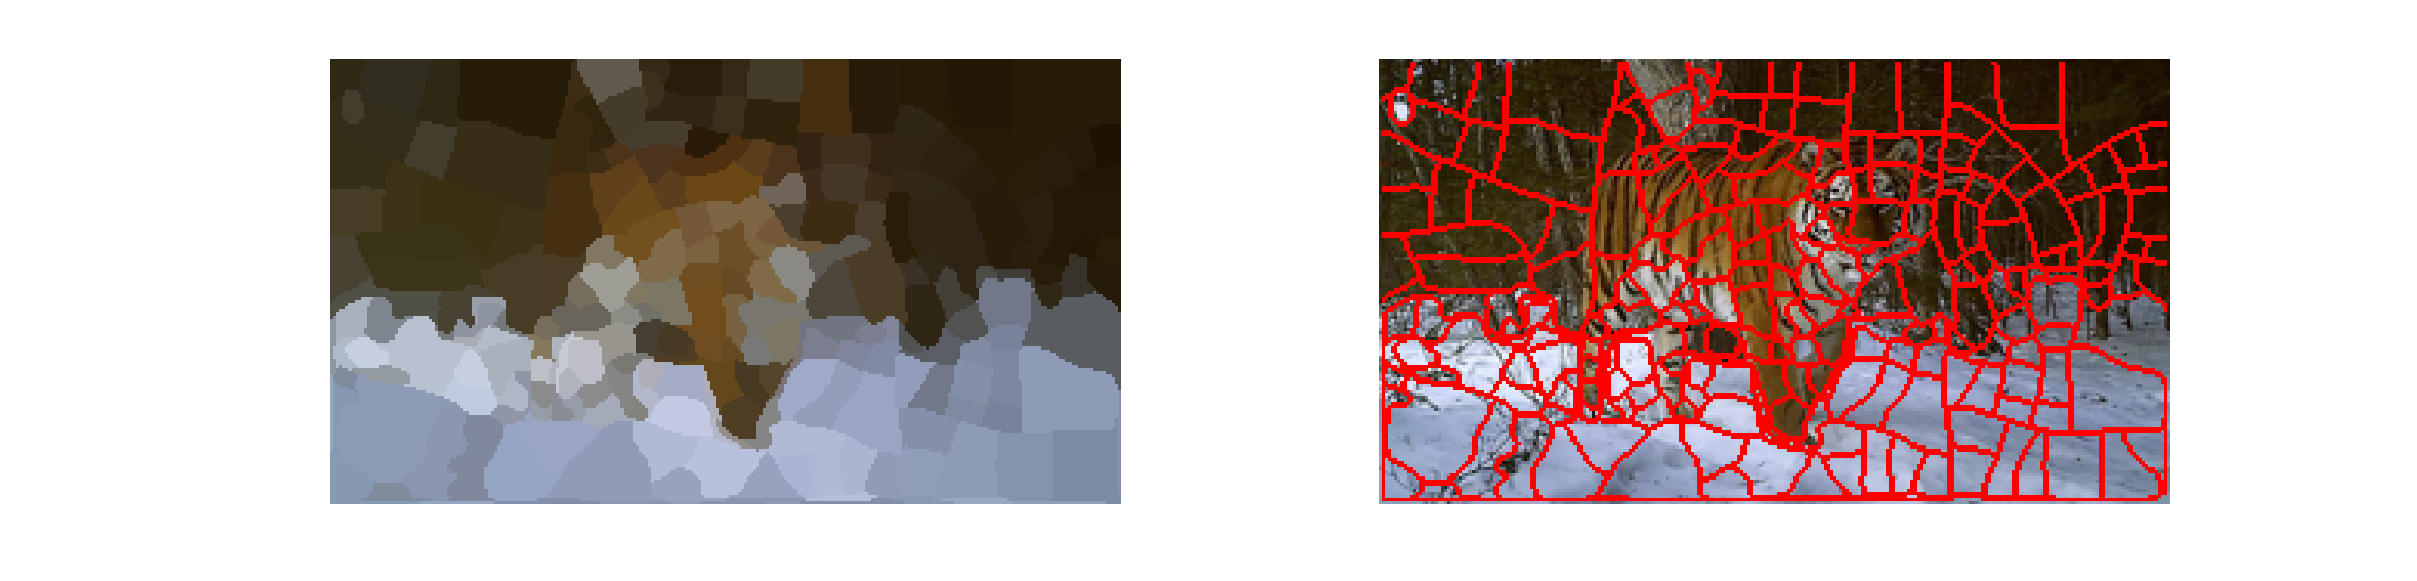
\includegraphics[width=\columnwidth]{Figure/Normalizedcut_Tiger2_Minarea_20.eps}
			\caption{Normalized Cut segmented \texttt{tiger2} with changing \texttt{min\_area} to $20$.}
			\label{fig:Normalizedcut_Tiger2_Minarea_20}
		\end{figure}

		\par \texttt{max\_depth} determines the maximum number of recursion to apply the implementation. As illustrated in Figure \ref{fig:Normalizedcut_Tiger2_Maxdepth_2}, the lower the \texttt{max\_depth} is the less the segmentation would be and the less modes would the modes be found.

		\begin{figure}[!ht]
			\centering
			
\includegraphics[width=\columnwidth]{Figure/Normalizedcut_Tiger2_Maxdepth_2.eps}
			\caption{Normalized Cut segmented \texttt{tiger2} with changing \texttt{max\_depth} to $2$.}
			\label{fig:Normalizedcut_Tiger2_Maxdepth_2}
		\end{figure}

		\par Also, as illustrated in Figure \ref{fig:ormalizedcut_Tiger2_Colorbandwidth_50}, the increase in \texttt{colour\_bandwidth} would also result in the increase of modes found and the color complexity as well.

		\begin{figure}[!ht]
			\centering
			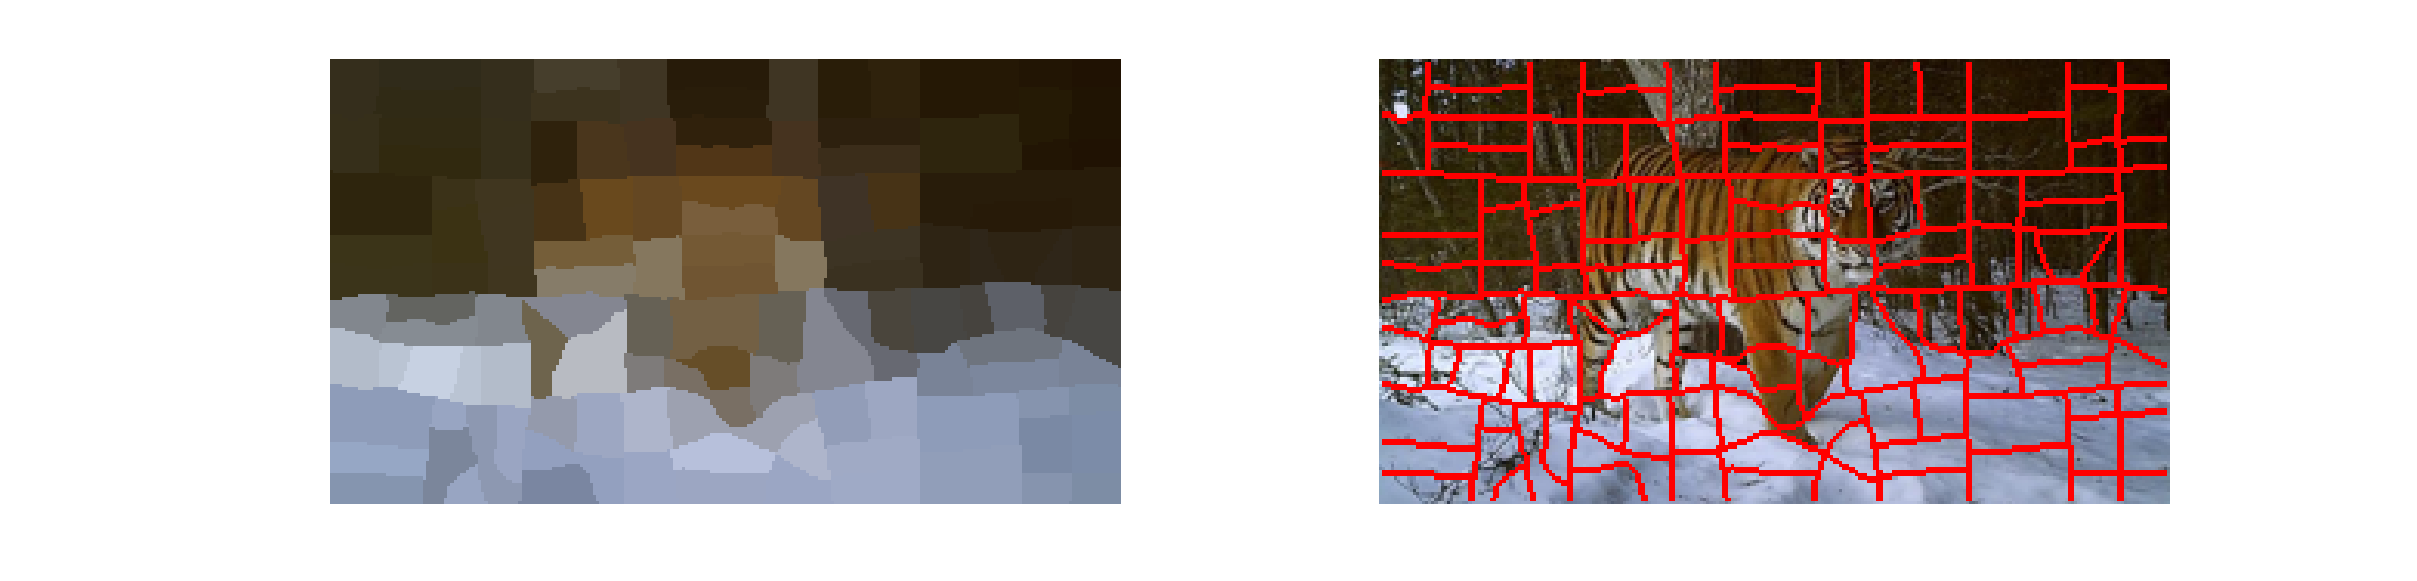
\includegraphics[width=\columnwidth]{Figure/Normalizedcut_Tiger2_Colorbandwidth_50.eps}
			\caption{Normalized Cut segmented \texttt{tiger2} with changing \texttt{colour\_bandwidth} to $50$.}
			\label{fig:ormalizedcut_Tiger2_Colorbandwidth_50}
		\end{figure}

		\par In Figure \ref{fig:Normalizedcut_Tiger2_Best_Result}, the best result for Normalized Cut segmentation of \texttt{tiger2} is shown. The parameters setting is \texttt{colour\_bandwidth} = $20.0$, \texttt{ncuts\_thresh} = $0.2$, \texttt{min\_area} = $10$, and \texttt{max\_depth} = $16$.

		\begin{figure}[!ht]
			\centering
			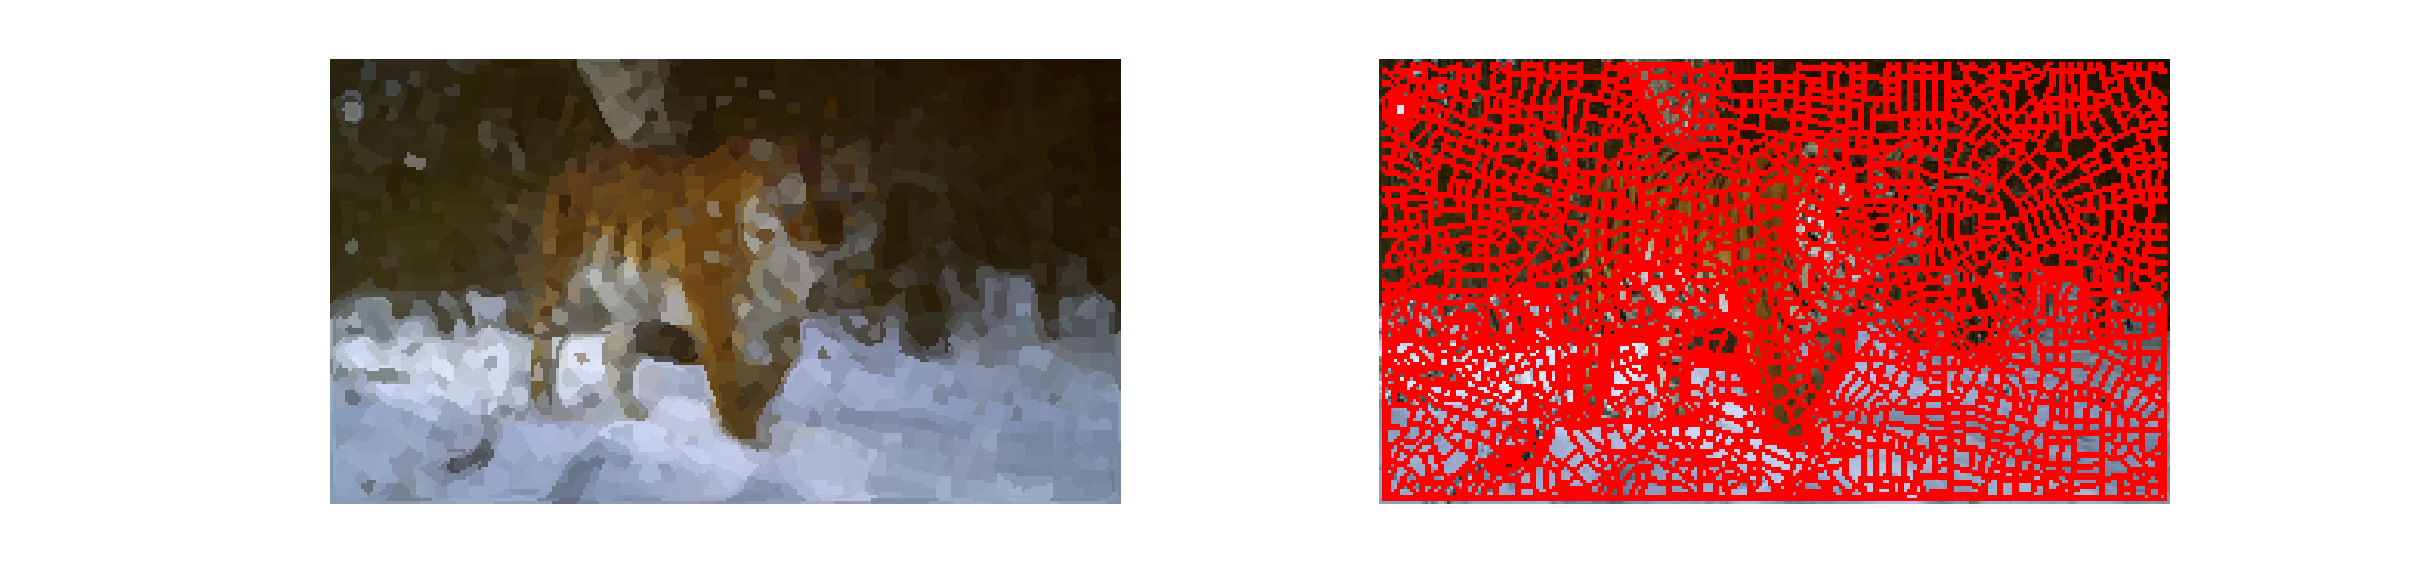
\includegraphics[width=\columnwidth]{Figure/Normalizedcut_Tiger2_Best_Result.eps}
			\caption{Best result of Normalized Cut segmented \texttt{tiger2} with parameters setting: \texttt{colour\_bandwidth} = $20.0$, \texttt{ncuts\_thresh} = $0.5$, \texttt{min\_area} = $10$, and \texttt{max\_depth} = $16$.}
			\label{fig:Normalizedcut_Tiger2_Best_Result}
		\end{figure}
	
	\item\addtocounter{Counter}{1}\underline{\textbf{Question \arabic{Counter}:}} Which parameter(s) was most effective for reducing the subdivision and still result in a satisfactory segmentation?
		\par \texttt{ncuts\_thresh}, \texttt{min\_area}, and \texttt{max\_area} are all effective for reducing the subdivision. However, to get resulting image with a satisfactory segmentation, the parameters \texttt{ncuts\_thresh} and \texttt{min\_area} are the most effective.
	
	\item\addtocounter{Counter}{1}\underline{\textbf{Question \arabic{Counter}:}} Why does Normalized Cut prefer cuts of approximately equal size? Does this happen in practice?
		\par Normalized Cut prefers cuts of approximately equal size. Based on the equation:
		\begin{align*}
			\mathrm{Ncut}(A,B) = \frac{\mathrm{cut}(A,B)}{\mathrm{assoc}(A,\mathcal{V})} + \frac{\mathrm{cut}(A,B)}{\mathrm{assoc}(B,\mathcal{V})}
		\end{align*}
		and the nature of symmetry, $\mathrm{Ncut}(A,B)$ would be minimized if $\mathrm{assoc}(A,\mathcal{V}) = \mathrm{assoc}(B,\mathcal{V})$. So if the pixels on the vertices $\mathcal{V}$ are similar to each other, the Normalized Cut would tend to cut the image to approximately equal size.
		\par In practice, if we set the parameter \texttt{colour\_bandwidth} to a big value which means we would have larger tolerace on the difference of color, as illustrated in Figure \ref{fig:ormalizedcut_Tiger2_Colorbandwidth_50}, the image would be segmented into many equal sized parts. When this value is small, the image in general would not likely to be segmented into segements with equal size.
	
	\item\addtocounter{Counter}{1}\underline{\textbf{Question \arabic{Counter}:}} Did you manage to increase \texttt{radius} and how did it affect the results?
		\par Increasing the value of \texttt{radius} would reduce the subdivision of the segmented image and the segmentation is good which is shown in Figure \ref{fig:Normalizedcut_Tiger2_Best_Result_Radius_6} and \ref{fig:Normalizedcut_Tiger2_Best_Result_Radius_9} with comparison to Figure \ref{fig:Normalizedcut_Tiger2_Best_Result}. What is expected is that, if we increase the \texttt{max\_depth} and decrease the \texttt{min\_area} when increasing the \texttt{radius} to get equal number of subdivision as the best result, the segmentation could be better.
		\begin{figure}[!ht]
			\centering
			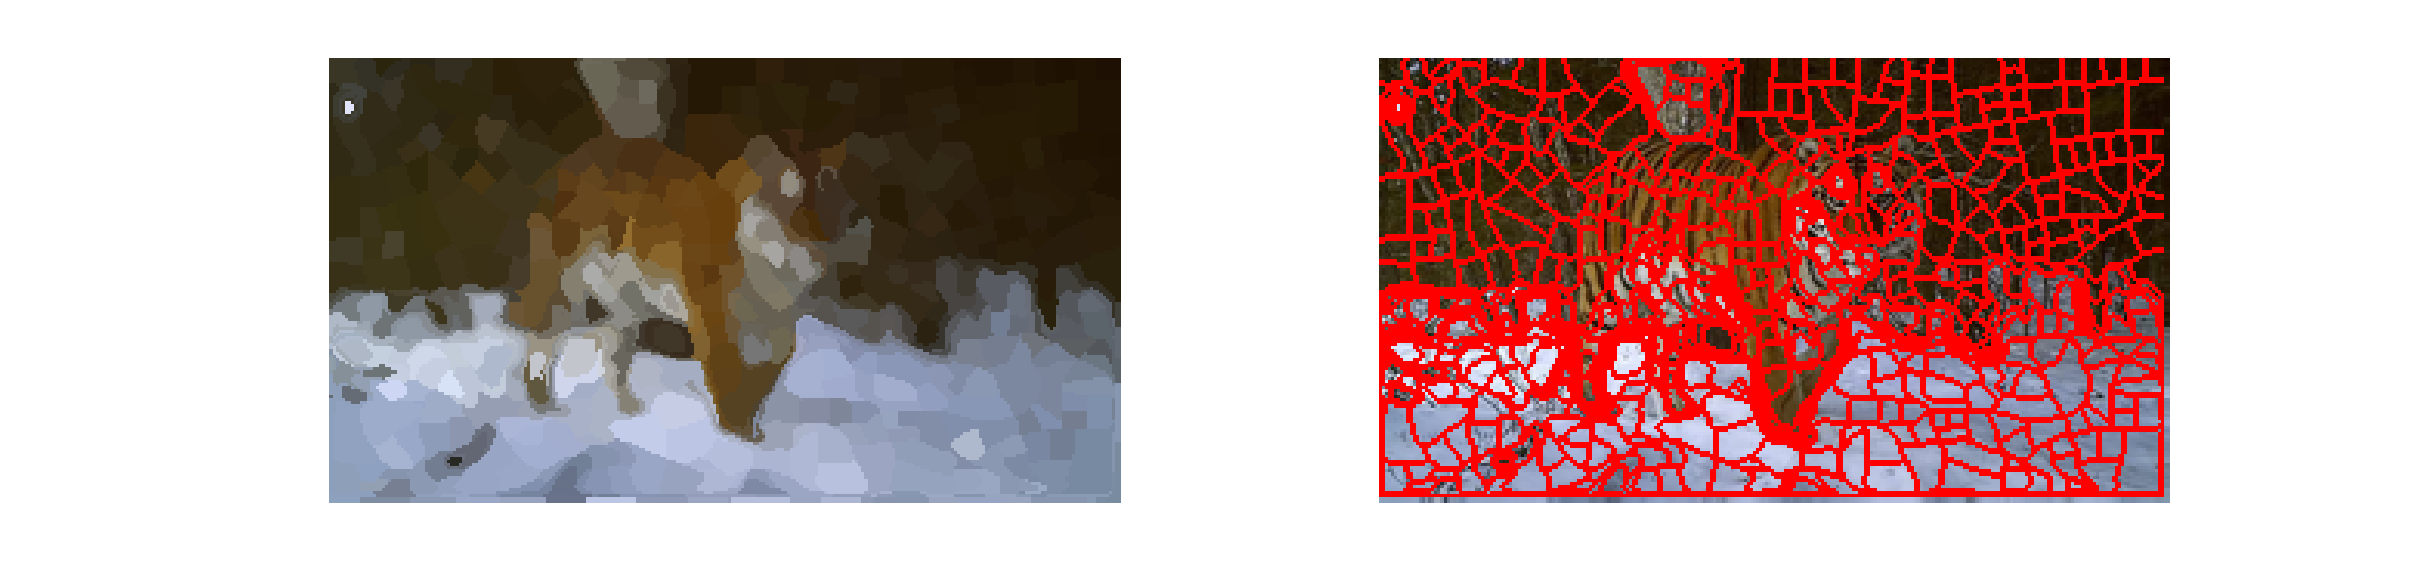
\includegraphics[width=\columnwidth]{Figure/Normalizedcut_Tiger2_Best_Result_Radius_6.eps}
			\caption{Best result of Normalized Cut segmented \texttt{tiger2} but change \texttt{radius} to 6.}
			\label{fig:Normalizedcut_Tiger2_Best_Result_Radius_6}
		\end{figure}
		
		\begin{figure}[!ht]
			\centering
			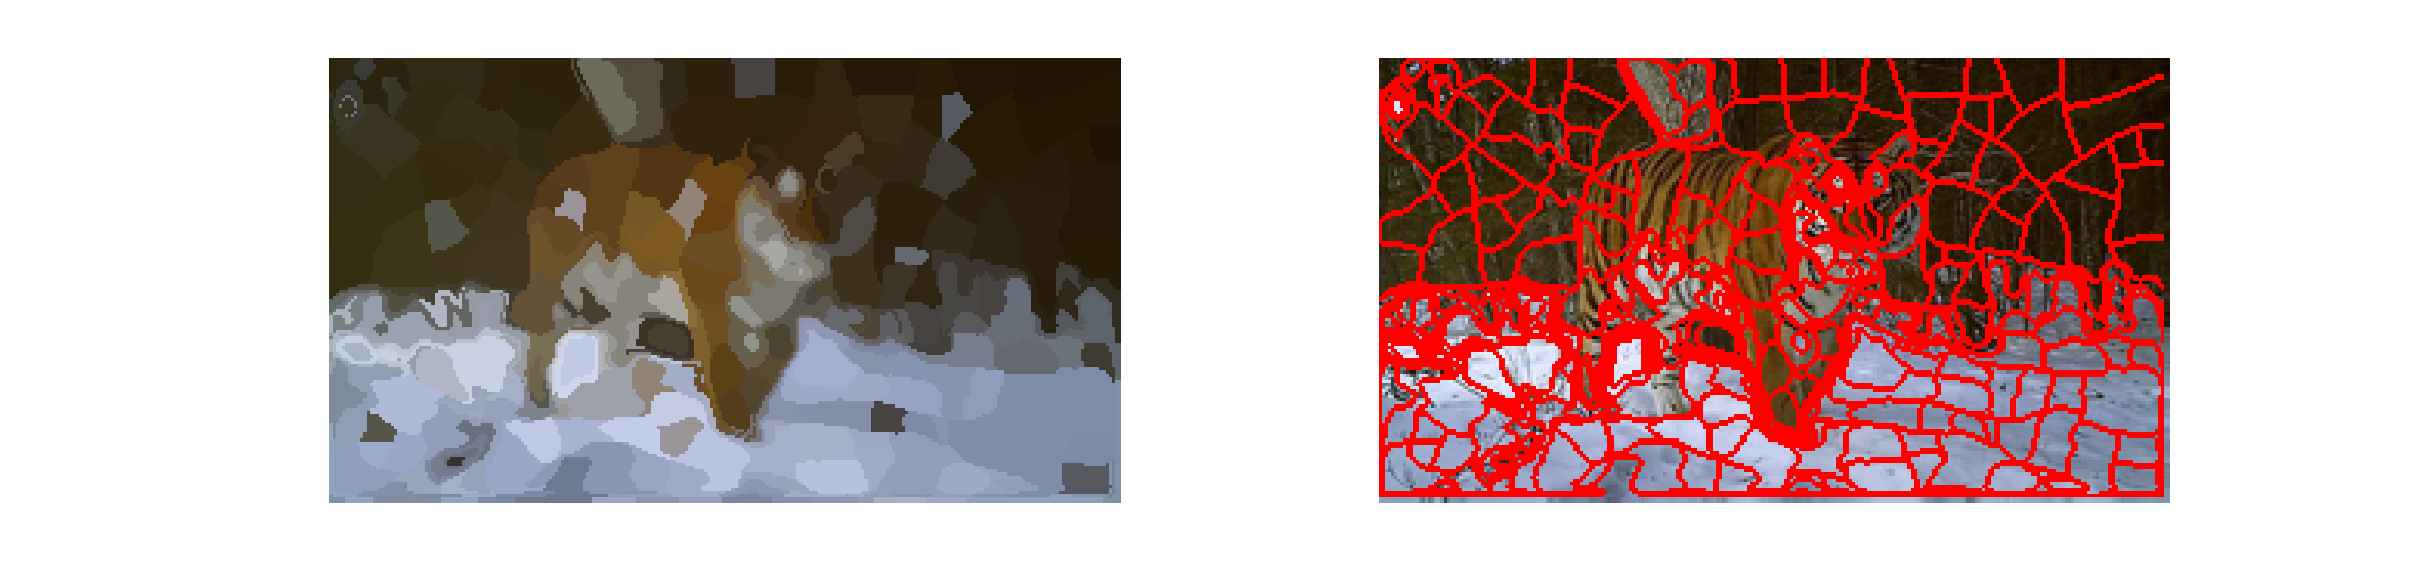
\includegraphics[width=\columnwidth]{Figure/Normalizedcut_Tiger2_Best_Result_Radius_9.eps}
			\caption{Best result of Normalized Cut segmented \texttt{tiger2} but change \texttt{radius} to 9.}
			\label{fig:Normalizedcut_Tiger2_Best_Result_Radius_9}
		\end{figure}
\end{itemize}

\section{Segmentation using graph cuts}
\begin{itemize}
	\item\addtocounter{Counter}{1}\underline{\textbf{Question \arabic{Counter}:}} Does the ideal choice of \texttt{alpha} and \texttt{sigma} vary a lot between different images? Illustrate with an example image with the parameters you prefer.
		\par The ideal choice of \texttt{alpha} and \texttt{sigma} doesn't vary a lot between different images. The ideal choice of \texttt{alpha} and \texttt{sigma} for image \texttt{tiger\_3} are $10$ and $16$ correspondingly with result illustrated in Figure \ref{fig:Graphcuts_Tiger3_Alpha_10_Sigma_16_K_16}.
		\begin{figure}[!ht]
			\footnotesize
			\centering 
			\begin{subfigure}[t]{0.49\linewidth} % Figure (a)
			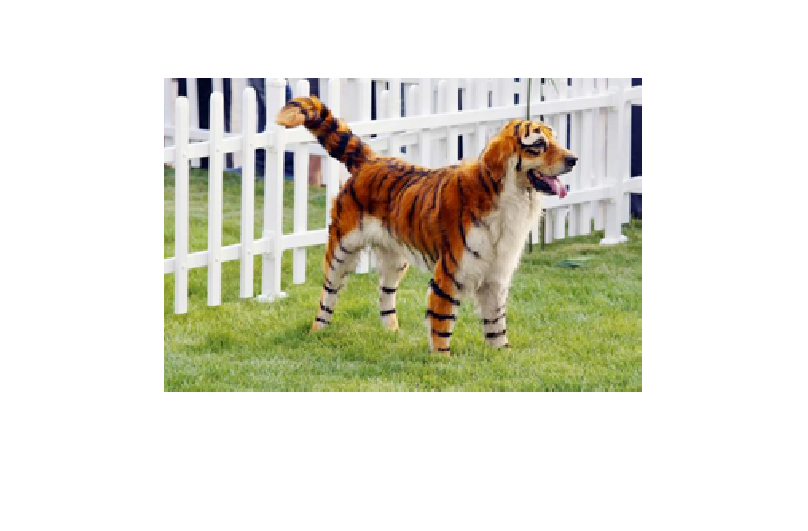
\includegraphics[width=\columnwidth]{Graphcuts0_Tiger3_Alpha_10_Sigma_16_K_16.eps}
			\caption{Original image of \texttt{Tiger\_3}.}
			\label{fig:Graphcuts0_Tiger3_Alpha_10_Sigma_16_K_16}
			\end{subfigure}
			\begin{subfigure}[t]{0.49\linewidth} % Figure (b)
			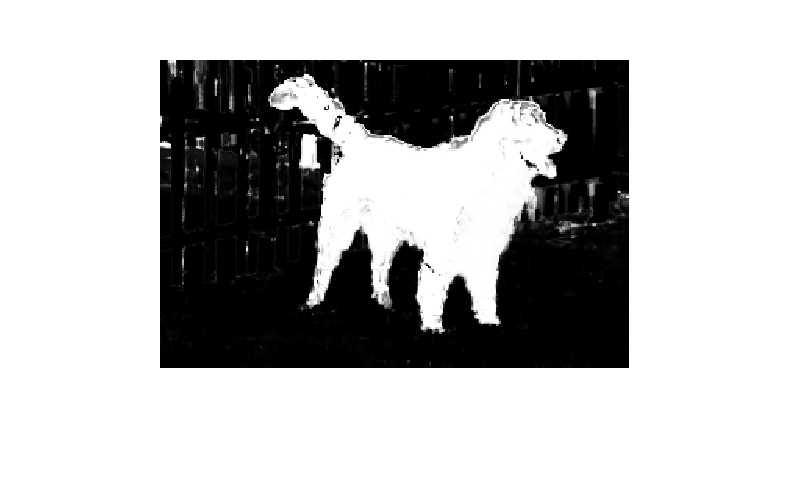
\includegraphics[width=\columnwidth]{Graphcuts1_Tiger3_Alpha_10_Sigma_16_K_16.eps}
			\caption{The likelihood for each pixels to be assigned to foreground.}
			\label{fig:Graphcuts1_Tiger3_Alpha_10_Sigma_16_K_16}
			\end{subfigure}
			\begin{subfigure}[t]{0.49\linewidth} % Figure (c)
			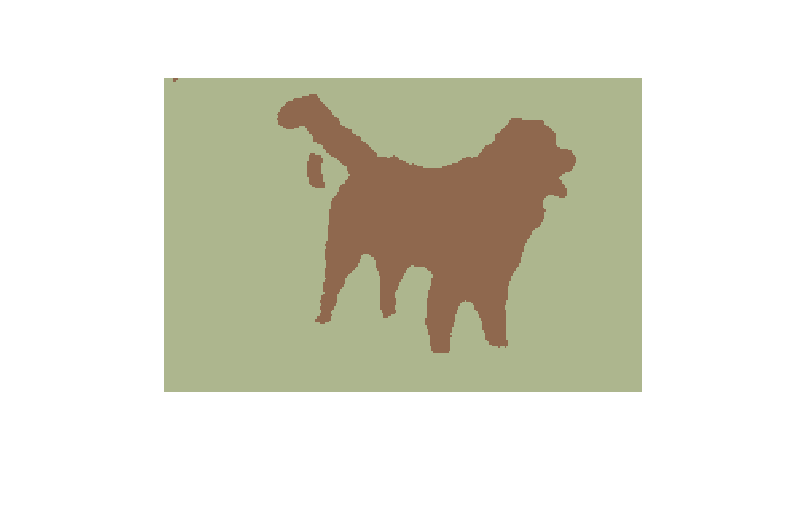
\includegraphics[width=\columnwidth]{Graphcuts2_Tiger3_Alpha_10_Sigma_16_K_16.eps}
			\caption{Threshold the likelihood to $0.5$.}
			\label{fig:Graphcuts2_Tiger3_Alpha_10_Sigma_16_K_16}
			\end{subfigure}
			\begin{subfigure}[t]{0.49\linewidth} % Figure (d)
			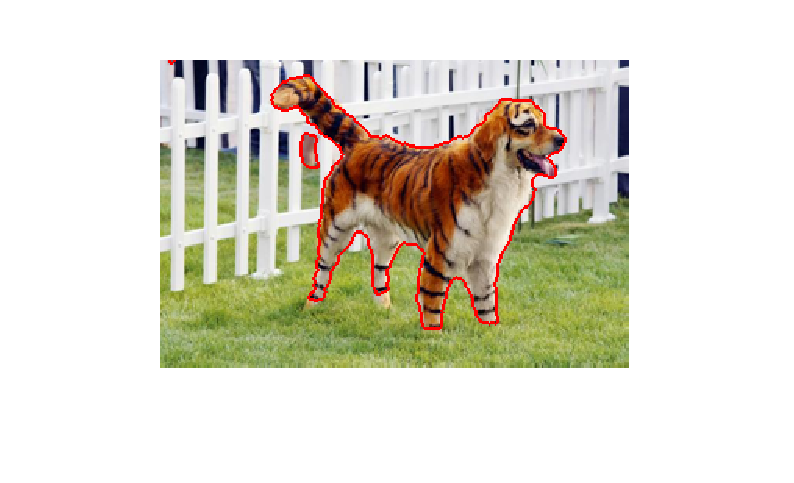
\includegraphics[width=\columnwidth]{Graphcuts3_Tiger3_Alpha_10_Sigma_16_K_16.eps}
			\caption{Result of segmentation.}
			\label{fig:Graphcuts3_Tiger3_Alpha_10_Sigma_16_K_16}
			\end{subfigure}
			
			\caption{Segmentation of \texttt{tiger\_3} using graph cuts with \texttt{alpha} $10$ and \texttt{sigma} $16$.}
			\label{fig:Graphcuts_Tiger3_Alpha_10_Sigma_16_K_16}
		\end{figure}
	
	\item\addtocounter{Counter}{1}\underline{\textbf{Question \arabic{Counter}:}} How much can you lower \texttt{K} until the results get considerably worse?
		\par When segmenting image \texttt{tiger\_3}, even if \texttt{K} is lowered to $2$, the result is still good enough for me.
		\par Take image \texttt{tiger\_1} as the example in this case, when \texttt{K} is lowered to $7$, the result is still good enough. While when \texttt{K} becomes to $6$, the result gets considerably worse, which is shown in Figure \ref{fig:Graphcuts_Tiger3_Alpha_10_Sigma_16_K_7_6}.
		\begin{figure}[!ht]
			\footnotesize
			\centering 
			\begin{subfigure}[t]{0.49\linewidth} % Figure (a)
			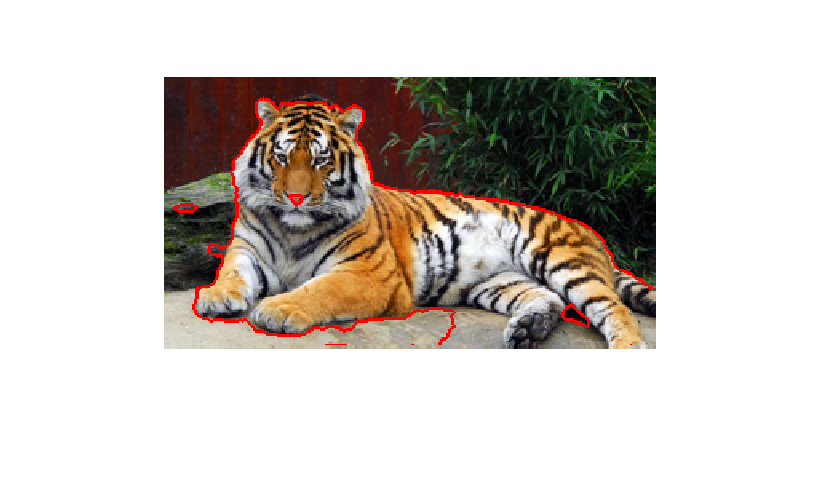
\includegraphics[width=\columnwidth]{Graphcuts_Tiger1_Alpha_8_Sigma_16_K_7.eps}
			\caption{Result of segmentation when \texttt{K} is $7$.}
			\label{fig:Graphcuts_Tiger1_Alpha_8_Sigma_16_K_7}
			\end{subfigure}
			\begin{subfigure}[t]{0.49\linewidth} % Figure (b)
			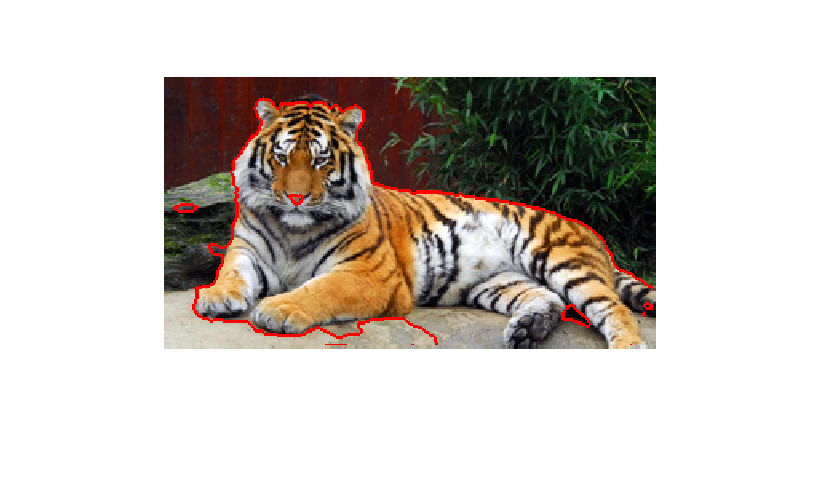
\includegraphics[width=\columnwidth]{Graphcuts_Tiger1_Alpha_8_Sigma_16_K_6.eps}
			\caption{Result of segmentation when \texttt{K} is $6$.}
			\label{fig:Graphcuts_Tiger1_Alpha_8_Sigma_16_K_6}
			\end{subfigure}
			
			\caption{Comparison between the result when \texttt{K} is $7$ and $6$.}
			\label{fig:Graphcuts_Tiger3_Alpha_10_Sigma_16_K_7_6}
		\end{figure}
	
	\item\addtocounter{Counter}{1}\underline{\textbf{Question \arabic{Counter}:}} Unlike the earlier method, Graph Cut segmentation relies on some input from a user for defining a rectangle. Is the benefit you get of this worth the effort? Motivate!
		\par The answer should depends on the context of what kind of segmentation we need. The Graph Cut segmentation worth the effort to deal with the images having clear background and foreground. Also, the Graph Cut is only useful when there is on object.
		\par However, when there is no obvious objects or difference between background and foreground, the Graph Cut does not worth all the changes.
	
	\item\addtocounter{Counter}{1}\underline{\textbf{Question \arabic{Counter}:}} What are the key differences and similarities between the segmentation methods (K-means, Mean-shift, Normalized Cut and energy-based segmentation with Graph Cuts) in this lab? Think carefully!!
		\par Differences:
		\begin{itemize}
			\item The K-means segmentation method we use in this lab only find the similarity of the pixels in the color domain, thus the output of K-means segmentation are seperated into different areas.
			\item Graph Cuts need prior information for better segmentation.
			\item Normalized Cut and energy-based segmentation with Graph Cuts view the images as graphs.
		\end{itemize}
		
		\par Similarities:
		\begin{itemize}
			\item All the segmentation methods are to find the similarities among the pixels and put the similar pixels into one segmentation.
		\end{itemize}
\end{itemize}

% Template
%%%%%%%%%%%%%%%%%%%%%%%%%%%%%%%%%%%%%%%%
%\begin{figure}[!ht]
%	\centering
%	\includegraphics[width=0.43\columnwidth]{xxx.eps}
%	\scalebox{0.9}{\input{xxx.tex}}
%	\caption{xxx.}
%	\label{fig:xxx}
%\end{figure}
%%%%%%%%%%%%%%%%%%%%%%%%%%%%%%%%%%%%%%%%
%\begin{figure}[!ht]
%	\footnotesize
%	\centering 
%	\begin{subfigure}[t]{.32\linewidth} % .32 for three polts .49 for two plots
%	
\includegraphics[width=\columnwidth]{Linearity_F.eps}
%	\caption{Image F}
%	\label{fig:F}
%	\end{subfigure}
%	\begin{subfigure}[t]{.32\linewidth} % .32 for three polts
%	
\includegraphics[width=\columnwidth]{Linearity_G.eps}
%	\caption{Image G = F'}
%	\label{fig:G}
%	\end{subfigure}
%	\begin{subfigure}[t]{.32\linewidth} % .32 for three polts
%	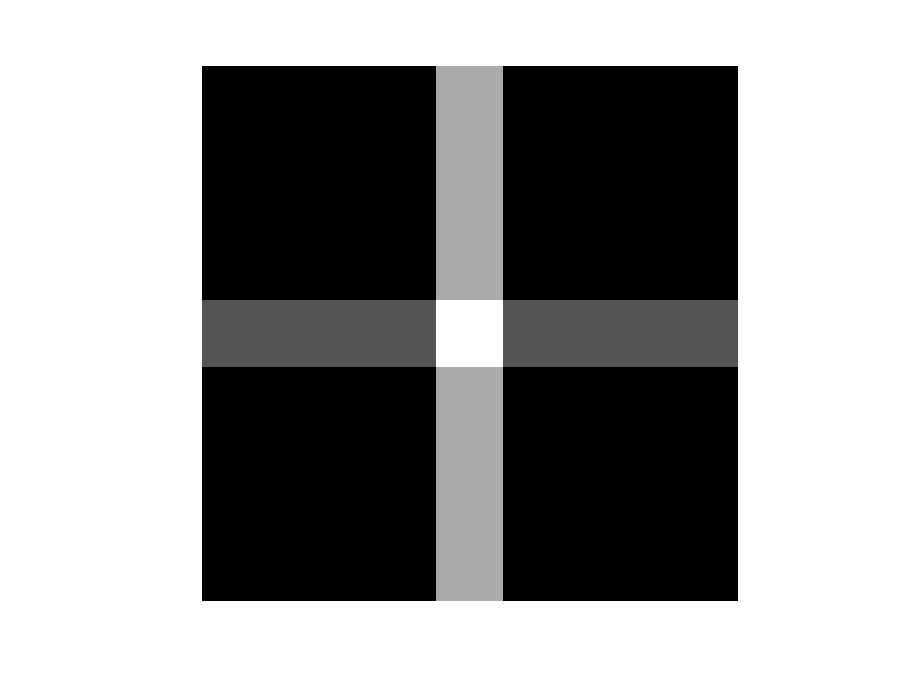
\includegraphics[width=\columnwidth]{Linearity_H.eps}
%	\caption{Image H = F + 2 * G}
%	\label{fig:H}
%	\end{subfigure}
%	\caption{Origin images.}
%	\label{fig:origin}
%\end{figure}
%%%%%%%%%%%%%%%%%%%%%%%%%%%%%%%%%%%%%%%%
%\begin{align*}
%	var_{t = 0.1} &= \begin{bmatrix} 0.0133 & 0.0000 \\ 0.0000 & 0.0133 \end{bmatrix} \\
%	var_{t = 0.3} &= \begin{bmatrix} 0.2811 & 0.0000 \\ 0.0000 & 0.2811 \end{bmatrix} \\
%	var_{t = 1.0} &= \begin{bmatrix} 1.0000 & 0.0000 \\ 0.0000 & 1.0000 \end{bmatrix} \\
%	var_{t = 10.0} &= \begin{bmatrix} 10.0000 & 0.0000 \\ 0.0000 & 10.0000 \end{bmatrix} \\
%	var_{t = 100.0} &= \begin{bmatrix} 100.0000 & 0.0000 \\ 0.0000 & 10.0000 \end{bmatrix}
%\end{align*}
%%%%%%%%%%%%%%%%%%%%%%%%%%%%%%%%%%%%%%%%
% \lstinputlisting{x.m}
%%%%%%%%%%%%%%%%%%%%%%%%%%%%%%%%%%%%%%%%
\end{document}